\section{Общие понятия. Первая теорема Абеля}\label{sec-power-series-01}

\begin{definition}[Степенной ряд]\label{def-power-series}

Ряд вида

\begin{equation}
\sum_{n=0}^\infty c_n(z-z_0)^n,
\qquad c_n,z_0\in\mathbb C,
\label{eq-power-series}
\end{equation}

называется степенным рядом с центром \(z_0\). В вещественном случае \(c_n,z_0,z\in\mathbb R\).

Сдвиг \(w=z-z_0\) сводит его к ряду \(\sum_{n=0}^\infty c_nw^n\) с центром в нуле.

\end{definition}

\begin{theorem}[Первая теорема Абеля]\label{thm-abel-first}

Для ряда \(\sum c_nz^n\):

\begin{enumerate}
\def\labelenumi{\arabic{enumi}.}
\tightlist
\item
  Если ряд сходится в точке \(a\ne0\), то он сходится абсолютно при \(|z|<|a|\) и равномерно на каждом замкнутом круге \(|z|\le r<|a|\).
\item
  Если ряд расходится в точке \(b\), то он расходится при всех \(|z|>|b|\).
\end{enumerate}

\end{theorem}

Весь открытый круг \(|z|<|a|\) не обязан быть множеством равномерной сходимости.

\begin{proof}

\textbf{1.} Из сходимости \(\sum c_na^n\) следует \(c_na^n\to0\), поэтому существует \(M>0\) с \(|c_na^n|\le M\) для всех \(n\). При \(|z|\le r<|a|\) положим \(q=r/|a|<1\). Тогда \[
|c_nz^n|=|c_na^n|\left|\frac za\right|^n\le Mq^n.
\] Ряд \(\sum Mq^n\) сходится. По теореме \ref{thm-weierstrass} получаем равномерную сходимость на \(|z|\le r\) и абсолютную в каждой его точке. Любая точка \(|z|<|a|\) попадает в такой круг.

\textbf{2.} Если бы ряд сходился в точке \(z_1\) с \(|z_1|>|b|\), то по первой части он сходился бы в \(b\). Противоречие.

\end{proof}

\begin{definition}[Радиус сходимости]\label{def-radius}

Радиус сходимости ряда \eqref{eq-power-series} определяется как \[
R=\sup\left\{|w|:\ \sum_{n=0}^\infty c_nw^n\text{ сходится}\right\},
\qquad 0\le R\le+\infty.
\] При \(|z-z_0|<R\) ряд сходится абсолютно, при \(|z-z_0|>R\) расходится. На границе \(|z-z_0|=R\) требуется отдельное исследование.

В вещественном случае \((x_0-R,x_0+R)\) называется интервалом сходимости; его концы не включаются в это название независимо от сходимости в них.

\end{definition}

\begin{center}
\begin{minipage}{\linewidth}
\centering
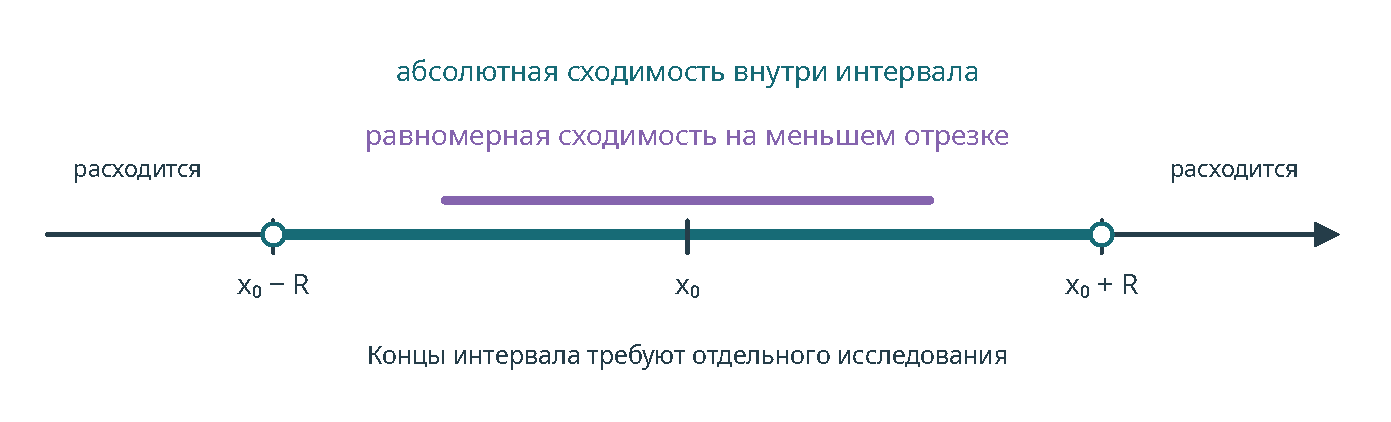
\includegraphics[width=0.95\linewidth]{figures/interval.pdf}
\captionof{figure}{Интервал сходимости и меньший отрезок равномерной сходимости.}\label{fig-interval}
\end{minipage}
\end{center}
